%% ----------------------------------------------------------------------------------
%% GUIDELINES
%% ----------------------------------------------------------------------------------
%% - Provide details about techniques/methods that you use. Do not just write “We have
%% implemented the marching cubes algorithm”. Describe the method too, in your own
%% words. Even if it is well described in a book, you should still explain the method
%% yourself; this is part of the exercise. Also, the reader may not know the method, nor
%% can the reader be bothered to find the document that you are referring to.
%% - Discuss interesting implementation aspects, but do not include code fragments in the
%% text. Pseudo code is allowed, but mathematical formulas are preferred.
%% - Describe parameters of methods and explain which settings you used and why.
%% - Provide evidence that the method you have implemented actually works as intended.
%% - Explain how you designed a color map, a transfer function, or even your whole visualization
%% approach.

\section{Compositing}\label{sec:compositing}
The compositing raycaster uses the same implementation as MIP to iterate through the view ray.
The fundamental difference between the two raycasters is the calculation of the resulting ray color.
Where MIP uses the maximal voxel value on the ray, compositing raycaster uses a more complex calculation to determine its value.
The compositing raycaster takes all voxel values into account.
Our compositing raycaster is implemented with a front-to-back approach:\\
$C_{i}^{r} = C_{i-1}^{r} + \alpha_{i} c_{i} T_{i-1}^{r}$\\
$T_{i}^{r} = (1 - \alpha_{i}) T_{i-1}^{r}$\\
Where $i$ is the current iteration on the ray.
$C^{r}_{i}$ is the color of the ray so far, when all iterations are complete this is the resulting ray color.
$\alpha_{i}$ is the opacity of the current voxel.
$c_{i}$ is the color of the current voxel.
And finally $T^{r}_{i}$ is the transparency, this transparency is not used for the resulting transparency.
The ray color value has no transparency, but the transparency is used for the weight of each voxel in the ray.
The initial value of $T^{r}_{i}$ is $1$.
And the initial RGB values of $C_{i}^{r}$ are $0$ and the alpha is $1$, this alpha is not changed during the calculation.

As mentioned, the raycaster iterates from front to back.
At each iteration the color of the ray $C_{i}^{r}$ is summed together with the value of the current voxel.
The value of the voxel depends on three elements, which are all multiplied together.
The first two elements are the opacity and color of the voxel.
The final element is the transparency $T^{r}_{i-1}$.
After updating the color of the ray the new transparency $T^{r}_{i}$ is calculated.
The transparency is multiplied with ($1 - \alpha_{i}$), where $\alpha_{i}$ is the opacity of the current voxel.
So the value of the transparency decreases every time the voxel has a opacity greater than $0$.
The result of this approach is that voxels in the front are weighted more strongly in the calculation than voxels in the back.
In figure \ref{fig:compositing} the result of our raycaster is compared with the compositing raycaster shown in the assignment, the resemblance is clear.

\begin{figure}[h!]
    \centering
    \captionsetup{justification=centering,margin=0.5cm}
    \begin{subfigure}[t]{0.4\textwidth}
        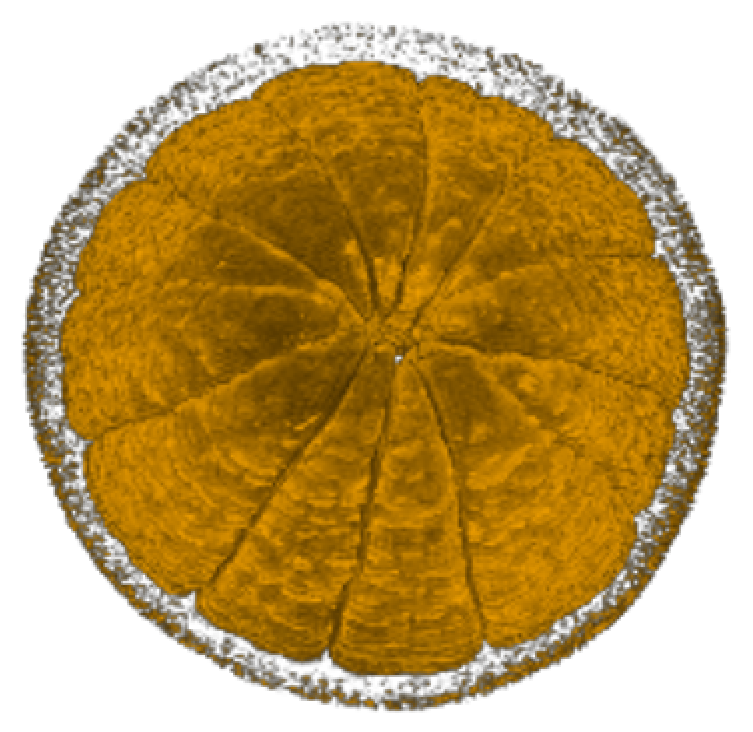
\includegraphics[width=\textwidth]{img/orange-them.png}
        \caption{ }
    \end{subfigure}
    \begin{subfigure}[t]{0.4\textwidth}
        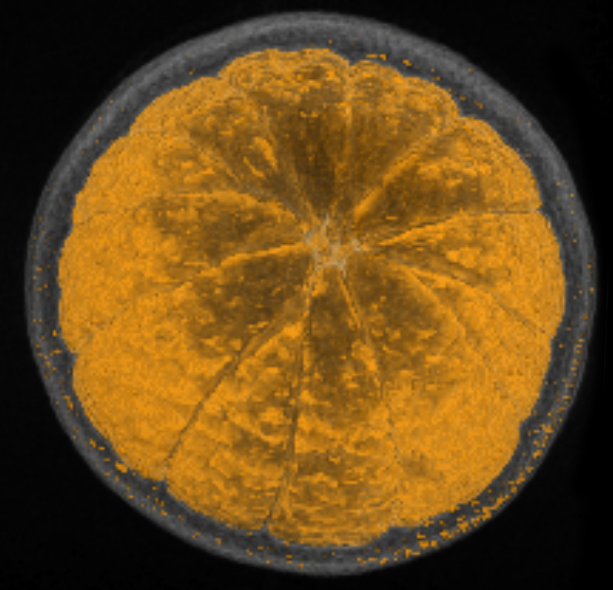
\includegraphics[width=\textwidth]{img/orange-us.png}
        \caption{ }
    \end{subfigure}
    \caption{Difference between the orange in the assignment (a) and ours (b)}
    \label{fig:compositing}
\end{figure}

\subsection{Comparison with MIP}
For the comparison between the two raycasters we implemented radio buttons to easily switch between them.
This was very convenient because we could instantly switch using the same settings and view angle.

The resulting visualizations between both raycasters differ a lot, as shown in figure \ref{fig:compareraycasters}.
The compositing raycaster, shown in (a), clearly shows multiple layers.
Whereas the MIP does not show any layers, it only shows the outside because it has the highest density.
When we change the opacity of this density range to 0 only the outline of the piggy bank remains visible, shown in (c).
So with MIP it is impossible to show the coins that are inside the piggy bank. 
With MIP you can see the patterns that are on the outside of the piggy bank, they appear to be flowers.
In the compositing raycaster this is a lot harder to make this visible.

\begin{figure}[h!]
    \centering
    \captionsetup{justification=centering,margin=0.5cm}
    \begin{subfigure}[t]{0.32\textwidth}
        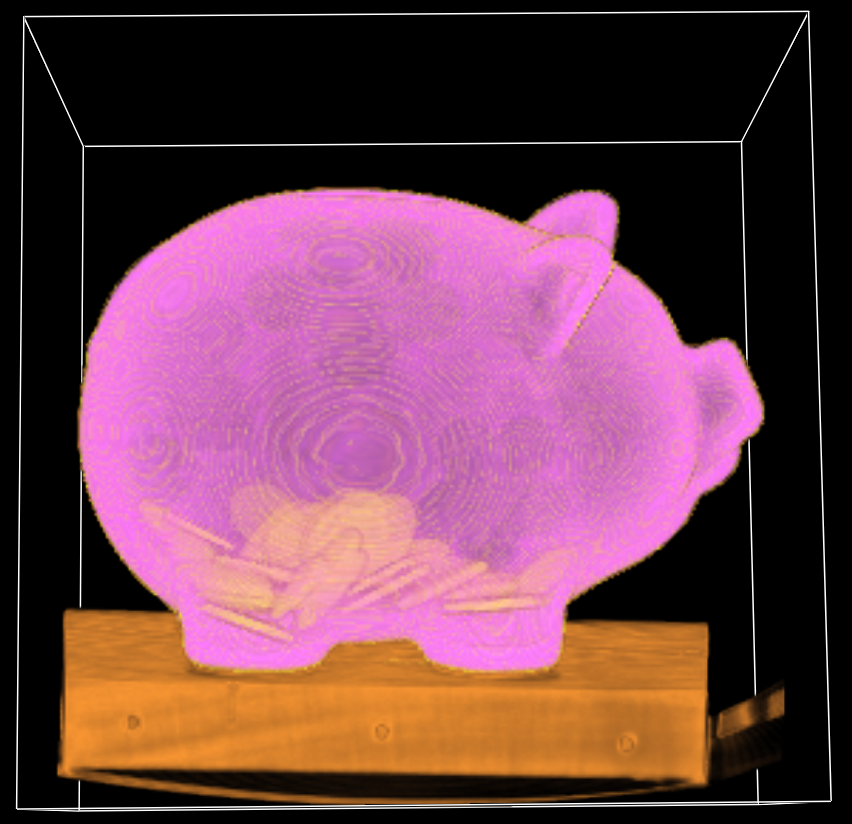
\includegraphics[width=\textwidth]{img/pig-compositing.png}
        \caption{ }
    \end{subfigure}
    \begin{subfigure}[t]{0.32\textwidth}
        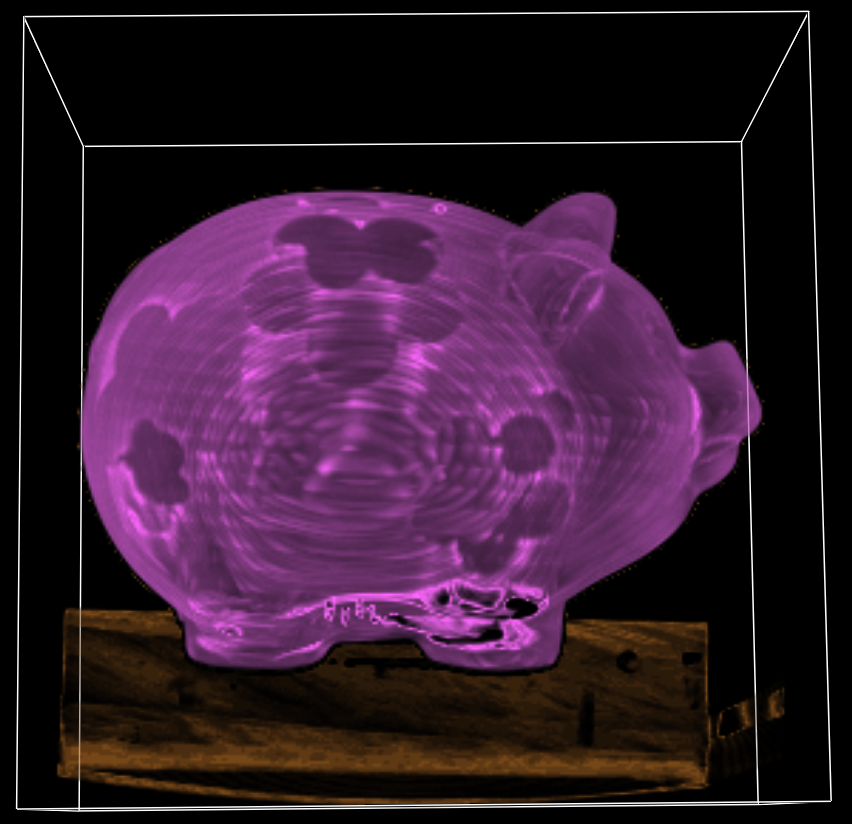
\includegraphics[width=\textwidth]{img/pig-mip.png}
        \caption{ }
    \end{subfigure}
    \begin{subfigure}[t]{0.32\textwidth}
        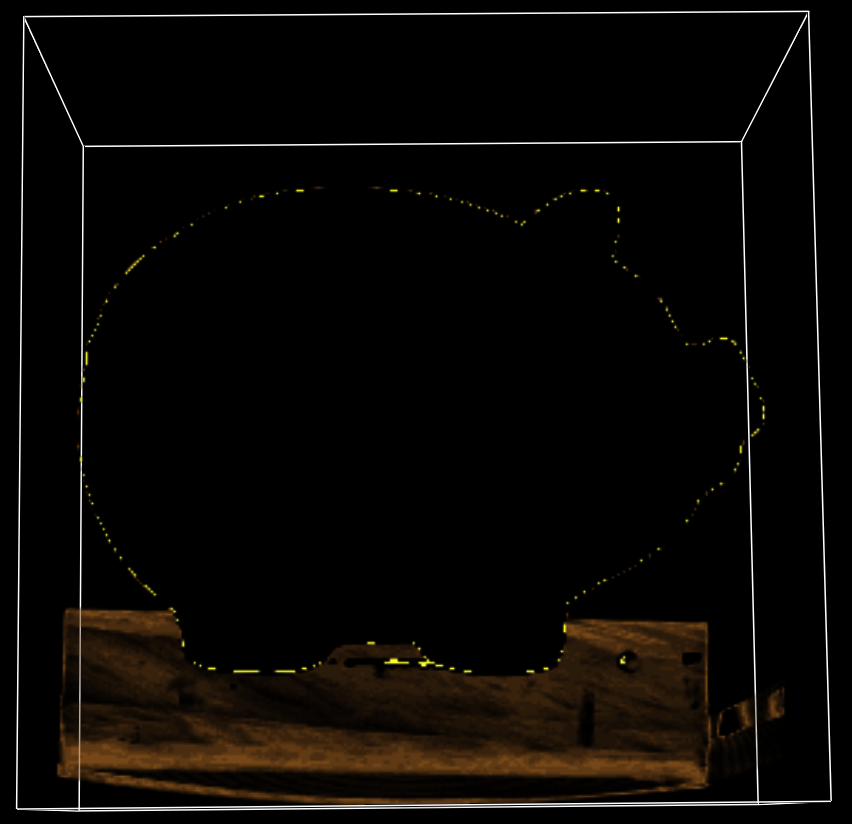
\includegraphics[width=\textwidth]{img/nopig-mip.png}
        \caption{ }
    \end{subfigure}
    \caption{(a) Rendering with compositing raycaster, (b) and (c) rendering with MIP raycaster}
    \label{fig:compareraycasters}
\end{figure}


